\documentclass[titlepage]{article}
\usepackage[T1]{fontenc}
\usepackage[utf8]{inputenc}
\usepackage[english]{babel}
\usepackage{graphicx}


\author{Luca Massini \and Daniele Nicolò}

\title{Requirement analysis and specification document
\\ Safestreets}

\date{release date to be defined}
\begin{document}
\maketitle
\newpage 
\tableofcontents
\newpage

\section{Introduction}
The purpose of this document is to represent the Requirement Analysis and Specification Document (RASD).
This document shows what are the goals and the requirements of the software.
It has to represent how the application can be useful for the users that will use it and why they are fundamental to improve the quality of the service offered. Secondly, this document can be also used as a support for the testing of the system, for the verification activities and also the validation ones. The RASD can be also used to guide the changes in a already existing system.
\subsection{Purpose}

\subsubsection{Description of the given problem:}
SafeStreets is a software useful to help people to be safer when they are on the street.\\
The users can send to the municipality pictures of violation occurring in public streets: the reporting can concern violation on the road, in a parking and so on.\\
The software allows the users to send detailed information about the violation, such as the hour, the date, the type of violation and the position (they can be captured with GPS).\\
Furthermore, the service can provide, both to the user and to the municipality,information about the streets in which the user is around,
such as the number of violations per street and consequently the level of danger of the street.\\
In addition, the user can have a different service based on the category to which he/she belongs.\\
The user and the municipality can also find on the application the most “dangerous” vehicles, that are the ones with the highest number of reports from the users.\\
The service must be different in base of the type of user, such  authorities, motorists, motorcyclists, bikers, pedestrians, disabled people, etc, so it must be easy to use.\\
Finally, the users must be able to receive recommendations from the system to avoid using streets, parking lots that are risky in general or at a specific hour or date.\\

\subsubsection{Goals:}
\begin{itemize}
\item $[goal 1]$:  The service allows the users to report a violation to the municipality.
\begin{itemize}

	\item $[goal 1.1]$: The user can send a picture of the 			violation.
	
	\item $[goal 1.2]$: The user can specify the date and the 						hour when the violation has happened 							and the type of violation.
	

	\item $[goal 1.3 ]$: The municipality must be able to     	receive the reports  \\
	
\end{itemize}

\item $[goal 2]$: The service allows the users to have detailed information about the violations and the street safety.
      \begin{itemize}
      	\item $[goal 2.1]$: The users can know which are the 			most reported streets, areas or parking.
      	
      	\item $[goal 2.2]$: The users can see which are the 				vehicles that commit the highest number
		of traffic violations.
		
		\item $[goal 2.3]$: The user, in base of his/her 				position, can be recommended to use the safest 					streets/areas, etc or avoid the dangerous ones, that 			are highlighted in different ways on the map.\\

      \end{itemize}
\item $[goal 3]$: The service offers different types of 						  interfaces and accessibility in according 					  to the type of user (biker, pedestrian, 						  rider, driver, disabled person).
	\begin{itemize}
	\item $[goal 3.1]$: The user that want to park his/her  							car/motorbike can receive a                           						suggestion of where to do it 
						based on the safest streets around 								him/her.\\
	\end{itemize}


\item $[goal 4]$: A user can specify the category to which 						  he/she belongs (motorcyclist, biker, 							  pedestrian, car driver, disabled person) in 				  order to improve the service quality.\\

\item $[goal 5]$: A driver or a motorcyclist can add to his 					  personal profile the license plate of his 					  vehicle.\\

\item $[goal 6]$: Safestreets can send to the municipality 						  suggestions of what to do in order to 						  improve the safety on the streets for every 
				  type of Safestreets user.
	\begin{itemize}
	\item $[goal 6.1]$: The municipality must receive every 
					    suggestion sent by Safestreets.\\
					   
	
	\end{itemize}
\item $[goal 7]$: The user must be able to sign-up into the safestreets platform.
\item $[goal 8]$: The user must be able to log-in into the system after having done the sign-up.
\item $[goal 9]$: The user must be able to log-out of the system if logged-in.
\end{itemize}

\subsection{Scope:}
In this section is introduced the so called "world and machine phenomena".\\
We distinguish the world and the machine. The world is related to every phenomena that take place outside of the region of events that the system to be developed (called machine) is able to control or eventually observe. Instead, the machine is related to phenomena which happen inside the machine and so they're completely controllable. Some of the totality of the phenomena can be observed by the machine but they're controlled by the world and vice versa. These are called shared phenomena. In this section there will be described only the world phenomena and the shared one.The machine phenomena will be described later in the next chapters.

\paragraph{World phenomena: }
\subparagraph{From the user point of view: }
\begin{itemize}	
	\item The user sees one or more violations.
	\item The user wants to report a violation to the 					  municipality.
	\item The user wants to know the area/streets where the 
	     major violations occur.
	\item The user wants to know where is safer to park his/			  her car/bike/motorcycle.
	\item The user wants to know what are the vehicles that       		  commit the major number of violations.

\end{itemize}
\subparagraph{From the municipality point of view: }

\begin{itemize}
	\item The municipality wants to know what to do to 				improve the safety of the streets.
	\item The municipality wants to discover which are the most
	dangerous zones of the city.\\
\end{itemize}
 
\paragraph{Shared phenomena: }
\subparagraph{Shared phenomena controlled by the world and observed by the machine: }
\begin{itemize}
    \item The user signs-up into the platform.
    \item The user logs-in to the platform.
    \item The user logs-out from the platform.
 	\item The user sends to the system a picture of a            	violation and all the other data related to it.
 	\item The user sends some data request to the system.
	\item The municipality sends a data request to the system 		  in order to receive suggestion to improve the 				  safety 	of the streets.
	\item The municipality sends a data request to know what 			  are the vehicles that have committed the major 				  number of violations.
\end{itemize}
\subparagraph{Shared phenomena controlled by the machine and  			observed by the world: }
\begin{itemize}
	\item The user receives ,by the system,all the data 			related to the safest and most dangerous streets .
	\item The user receives, by the system, all the data related to the vehicles that have committed the major number of violations.
	\item The municipality receives suggestions from SafeStreets to provide a better 			safety on the streets.
	\item The municipality receives the list of the most 			dangerous vehicles .
	
\end{itemize}
\subparagraph{Machine phenomena: }
\begin{itemize}
	\item The system stores the user's data.
	\item The system stores all the data about the 					municipality.
	\item The system stores all the data about the violation.
	\item The system analyses the received picture in order to 	retrieve the car plate.
	\item The system checks if the street in which the 				violation occur is an existing street.
	\item The system runs an algorithm to retrieve suggestions from users' reports in order to provide them to the municipality.
\end{itemize}

\subsection{Definitions, Acronyms, Abbreviations}




\subsubsection{Acronyms:}

\begin{tabular}{|l|rl|}
\hline

\textbf{S2B}	& System to be 	&				 			 \\
\textbf{GDPR}	& General Data Protection Regulation &	     \\
\textbf{FC}     & Fiscal Code    	sign-up	&	 				 \\
\textbf{WP}     & World Phenomena       &	 				 \\
\textbf{MP}     & Machine Phenomena     &	 				 \\
\textbf{SP}     & Shared Phenomena      &     				 \\
\textbf{GPS}    & Global Positioning System &	 			 \\

\hline
\end{tabular}

\subsubsection{Definitions:}
\begin{itemize}
	\item \textbf{Violation =} Any kind of infringement of the highway code. Here we distinguish violations concerning the traffic and violation concerning parking.\\
	\item \textbf{Personal data =} Data belonging to the user, needed in the moment of the signing-up. They are name, surname, date of birth, e-mail and FC.
	\item \textbf{S2B =} System to be developed. It will contain all the services provided by SafeStreets.
	\item \textbf{Private user request =} A user can ask for information about the safety of an area or a parking lot around him/her. He/She can also request data about the most dangerous vehicles in that area.
	\item \textbf{Report of a violation =} A user can use SafeStreets to report an infringement he has seen. In particular he can add the type of violation, the date and the hour, the street (that can also be retrieved automatically) and he can also add a picture of the violation.
	\item \textbf{Municipality request =} The municipality can ask for the same things aforementioned for the user. They will receive more accurate information rather than a private user, including for example data about the violators. They can also request suggestions (provided by SafeStreets) to improve the quality of their service.
	\item \textbf{Fiscal code =} It's a 16-characters code identifying an Italian citizen.
	\item \textbf{Credentials =} username and password used by a user to log-in to the system.
	
\end{itemize}
\subsubsection{Abbreviations:}

\begin{itemize}

	\item Gn = n-th goal;
	\item Dn = n-th domain assumption;
	\item Cn = n-th constraint;
	\item Rn = n-th requirement;
	\item MP = Machine Phenomena;
	\item WP = World Phenomena;
	\item SP0 = Shared Phenomena that are managed by the Machine but that are observable by the World;
	\item SP1 = Shared Phenomena that are managed by the World but observable by the Machine.

\end{itemize}


\subsection{Revision History: }

\begin{itemize}

	\item Work started 13/10/19;

\end{itemize}

\subsection{Reference Documents:}
\begin{itemize}
	\item RASD Slides by professor Matteo Rossi (Polimi);
\end{itemize}
\subsection{Document Structure: }
This document is organized in the following way:
\begin{itemize}
	\item \textbf{Overall Description:} This section contains a deeper analysis of the world and machine phenomena already described in the scope. It also contains class diagrams which describe the relationship between actors, state chart diagrams used to describe the state of the system from a dynamic point of view, the description of the stakeholders and their needs and finally the key functional requirements and the domain assumption.
	
	\item \textbf{Specific requirements:} In this section there is a more detailed description of the requirements already described in the previous section. This is thought to help the develop team to understand what the system must ensure.In particular in this part there is a description of the external interfaces requirements,of the functional requirements, of the performance requirements, of the design constraints and finally of the software system attributes.
	
	\item \textbf{Formal analysis:} This section contains the formal analysis written in alloy. Alloy is a formal notation used to specify model of systems and software. Thanks to alloy it is possible to write a formal models with their own requirement, domain assumptions and goals and then check the correctness of the model.\\
There is another very important aspect concerning this section. Such aspect is the fact that alloy gives the possibility to clarify aspects that could be ambiguous. The ambiguity is usually and intrinsically due to natural language. 
\end{itemize}
\newpage

\section{Overall Description}
This section is necessary to give a better and deeper description of the shared and world phenomena. In this section, the system will be described also with the help of the class diagrams and state diagrams.
\subsection{Product Perspective:}
\paragraph{The user sees one or more violations:}
It's the situation in which the user sees a violation which can concern traffic or parking. The user knows what happens and also where and when. Such violations could be for example: a car/motorcycle parked in a red zone or on a sidewalk area or however any kind of traffic or parking violation.
\paragraph{The user wants to report a violation to the 					  municipality.}
In this case the user would like to have the possibility of report a violation of which he/she is aware. 
\paragraph{The user wants to know the areas/streets where the 
	      major number of violations occur.}
In this type of phenomena the user would like to know what are the most dangerous areas in his city/town in terms of traffic or parking violations. 
\paragraph{The user wants to know where is safer to park his/			  her car/bike/motorcycle:}
In this case we analyse the case in which the user has a vehicle that needs to be parked. He/she would know what are the safest streets in order to decide in which street to park. He/she wants to know the safest street whose distance from him/her is less than or equal to a certain value (given by the user).
\paragraph{The user wants to know what are the vehicles that       		  commit the major number of violations:}
The user would like to know the vehicles that commit the highest number of violations. Obviously, the user is not an authority and so he can see a limited quantity of information due to GDPR regulation.
\paragraph{The municipality wants to know what to do to 				improve the safety of the streets: }
In this case the municipality recognizes that in a certain area or street there is a problem with the too high number of violations. In this case the municipality would like to have some suggestions in order to provide a solution to make the number of violations decrease.
\paragraph{The municipality wants to discover what're the most dangerous zones of the city.}
The municipality would like to know which are the most dangerous streets in order to monitor them with more attention. This could be useful for the municipality if it wants to improve its service quality.
\paragraph{The user signs-in to the platform: }
In this case the user compiles all the mandatory fields which are: name,surname,username,password,fiscal code. Driving license data are not mandatory because this system is designed for people who use the app also to ride a bike or walk.
\paragraph{The user signs-up to the platform: }
In this case the user compiles all the mandatory fields which are: name,surname,username,e-mail,password and FC. Driving license data are not mandatory because this system is designed for people who use the app also to ride a bike or walk.
\paragraph{The user logs-in to the platform: }
The user can log-in to the system by entering username and password.
\paragraph{The user logs-out from the platform:}
In this case the user quits the platform if he/she logs-out. The user will not be able to receive any service  by the platform until he/she does a new log-in.
\paragraph{The user sends to the system a picture of a            	violation and all the other data related to it: }
In this case the user sends a report of a park violation or a traffic violation to the authorities (the municipality in this case). The user can take a picture of the violation and add the mandatory information which are needed which are: the hour and the date. The place of the violation can be detected automatically or manually (it's a user's choice).
\paragraph{The user sends some data request to the system: }
In this case the user could want to retrieve some information from the system. Such information, could concern the most dangerous zones or who commits the major number of violations, the most safe streets where to park and so on. The system will provide these information in different ways, such as a list of the users or a maps with the highlighted streets.
\paragraph{The municipality sends a data request to the 				   system  in order to receive suggestion to improve 			   the 	safety 	of the streets: }
The municipality sends a data request to the system in order to have suggestions to improve the safety. These suggestions are simple phrases which describe what it's possible to do to overcome problems.
\paragraph{The municipality sends a data request to know what 		   are the vehicles that have committed the highest 	         		  number of violations: }
In this case the authorities would like to understand which are the ones who commit the major number of violations, so they send a data request to retrieve those information. The municipality has to specify the types of vehicles (motorbikes, cars or every kind of vehicle that has a license plate), the maximum number of instances to obtain with the query.
\paragraph{The user receives from the system all the data 			related to the safest and most dangerous streets : }
In this case the user receives all the data about the streets that are considered the most dangerous or the safest. He/She receives a map with the highlighted streets which are at a certain distance from a point specified by the user.
\paragraph{The user receives from the system all the data related to the vehicles that have committed the major number of violations:}
In this case the user receives the list of license plates that have committed the highest number of violations. The user receives a number of license plates less than or equal the number he/she has specified as input.
\paragraph{SafeStreets provides the suggestion in order to give them to the authorities: }
SafeStreets runs an algorithm to retrieve information and suggestions about the future improvement of the streets safety from the users' reports. These data will be sent to the municipality so that they will be able to use them to enhance the safety.
\paragraph{The municipality receives suggestions to keep the streets safer: }
The municipality receives list where each element is composed on one side by the problem and on the other by the suggestion to overcome it.
\paragraph{The municipality receives the list of the most 			dangerous vehicles: }
The municipality receives all the license plates belonging to the vehicles that have committed the highest number of violations. The authorities select the maximum number of plates to receive (That they can choose each time as an input) and they obtain by the system a less than or equal number of license plates.
\paragraph{The system stores the user's data:}
The system will store permanently and safely all the user data. They will be stored in the system databases in such a way that data corruption is rather difficult.
\paragraph{The system stores all the data about the 					municipality:}
The system will also store all the data about the municipality in its databases.
\paragraph{The system stores all the data about the violation: }
The system will store all the information concerning the violation. Such information are the picture, the data, the hour, the license plate of the vehicle, and an unique identifier to distinguish identical violations eventually reported by different users.
\paragraph{The system analyses the received picture in order to 	retrieve the car plate: }
The system, after having received a picture of the violation, will run an algorithm to recognize the license plate of the vehicle that committed the violation so that it is uniquely identified. The algorithm takes the picture sent by the user as an input and works on it to retrieve the license plate. If it is recognizable from the picture, the system saves the data about it in its database. Otherwise it only keeps the information about the violation.
\paragraph{The system checks if the street in which the 				violation occur is an existing street: }
if the place of the violation is manually entered by the user there is the possibility that such place doesn't exist. In this case the system must automatically report an error to the user. Otherwise the system will store the street in the database together with all the other information related to the violation.
\subsection{Product functions: }
In this section there is a description of the main functions that the system will make available to the final user.\\
These functions are the following:
\begin{itemize}
	\item \textbf{Report of a violation:} Safestreets allows the user to report a violation. To do that he/she has to take a picture, indicate the hour and, eventually, the location where the violation occurred. The place where the violation occurred is taken automatically in case the user does not want to insert it himself, using the smartphone GPS signal. After that the violation will be reported to the municipality that will handle the problem.
	\item \textbf{Request of the list of vehicles that have committed the highest number of violations:}
	The users and the authorities can make a request and ask what are the vehicles that have committed the highest number of violations. This request (if no exception happen) will show a list of license plates to the user. The request can be personalized by expressing: a maximum number of vehicles that must be showed. If the number is not given as input the system will show a fixed number of results.
	\item \textbf{Get the list of most dangerous streets: }
	The most dangerous streets are the ones with the highest violations and they can be retrieved specifying the maximum number of vehicles that the request has to show. \\
Who is making the request has also to write the area of the streets he/she wants to analyse. This is done specifying the GPS coordinates of a fixed point and a maximum distance from that point. In this way, the user specifies a set of streets that he/she wants to analyse. The result of that request will be a map with the most dangerous roads highlighted.
	\item \textbf{Send a request to obtain suggestions to make the streets safer:}
	This function is only designed for the municipalities. In this case the municipality has to insert the place about which it wants to have suggestions. The system will return a list containing on one side the problem and on the other side a possible solution to overcome it. Obviously, the list is not static but it will be updated over time thanks to the reported violations.
	\item \textbf{The user send a request to know where to park his/her vehicle in a safe area:}
	This function allows the user to explicitly ask the system to suggest places where to park his vehicle in a secure way. 
The user must specify what type of vehicle he/she has and how far he/she wants to park from his/her position or from a position given as an input. The system will not guarantee the fact that in the proposed place there will be at least one parking lot but it only will suggest which roads are considered as more secure than others to do so.
	\item \textbf{The user will receive the suggested streets where to park:}
	After having requested the safest streets where to park, the system will provide them to the user in a map form. In this map there will be highlighted the streets considered more secure than the others in the specified area given by the user as input.

\end{itemize}
\subsection{User characteristics: }
In this subsection there is a description of the application users and an analysis of their needs. We will categorize the people who use the app in order to understand their necessities in a better way.\\
\textbf{\\Description of the users of the app:\\}
The user of the app can be divided in a first categorization which is the following:
\begin{itemize}
	\item Private user;
	\item Municipality or authority.\\
\end{itemize}
\textbf{Description of the private users: }\\ 
It is possible to divide again the private users in other classes. For every class there will be a different concept of dangerousness.
\begin{itemize}
	\item Pedestrians;
	\item Motorists;
	\item Motorcyclists;
	\item Cyclists.
\end{itemize}
A private user can be also a disabled person belonging to the pedestrians category or to the car drivers one. Because of this fact these type of users will require a different type of service and a different concept of dangerousness. For example they will have information about cars parked in a handicap parking or on ramps for disabled people.\\
All the private users are supposed to have downloaded the app from the store,to have done the sign-up entering all the mandatory data and finally to have accepted all the permissions.\\
The private user, according to his category, will take advantage of a different type of service.\\
A car driver, for example, will have information about parking lots or parking violation, that is not required in a biker service.\\
A cyclist will have informations about bicycle paths, while pedestrians will have detailed data about sidewalks or pedestrian crossing, with all the possible violations related to them. \\

Furthermore, the application can encounter:
\begin{itemize}
	\item Users that have downloaded the app but that haven't already signed-up in the system;
	\item Users that have already signed-up the system but that haven't logged-in yet. Users logged-out from the system belong to this category;
	\item Users also logged-in the system.\\
	
\end{itemize}

 



\subsection{Assumptions, dependencies and constraints: }
\subsubsection{Domain assumptions: }
\begin{itemize}
	\item $[\textbf{D1}]$: The user is supposed to submit correct e-mail, and data matching his/her fiscal code.
	\item $[\textbf{D2}]$: The user creates one and only one account.
	\item $[\textbf{D3}]$: Every municipality which has an account on the system certifies its own account as valid.
	\item $[\textbf{D4}]$: The GPS signal has a relative error of 10 meters.
	\item $[\textbf{D5}]$: The memory where the data is stored is persistent.
	\item$[\textbf{D6}]$: The user allows the app to have access to his/her position and the camera of his/her device.
	\item $[\textbf{D7}]$: The internet connection has to be enabled when the app needs it.
	
\end{itemize}
\subsubsection{Constraints: }
\begin{itemize}
	\item  The system must treat the users' personal data in according to the GDPR regulation.
	\item The system will be designed and implemented for smartphones.
	\item Since the system uses the fiscal code to identify the user it is supposed that it will be used only in Italy, so the application will have to be available only in the Italian app stores.
	\item The pictures must be taken only through the app camera and not imported from the device gallery in order to take photos in real time.
\end{itemize}

\subsubsection{Dependencies: }
\begin{itemize}
	\item The system will use the GPS services provided by the smartphones.
	\item The system will use the internet services offered by the smartphones.\\
\end{itemize}



\section{Specific Requirements}
\subsection{External Interface Requirements}
\subsubsection{User Interfaces}
\begin{itemize}
	\item\textbf{SafeStreet Interfaces}
	\begin{itemize}
		\item \textbf{SafeStreets Logo:}\\
		SafeStreets has a simple but explicative logo. It represents a street, because the main theme of the application concerns public roads. It also have a green tick, that represents the correct functioning and the safety of the streets.\\ \\ \\ \\ \\
		
	\begin{figure}[htbp]
	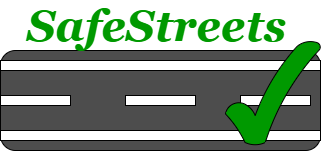
\includegraphics[scale=0.8]{Mockups/LogoSafeStreets.png}
	\centering
	\caption{SafeStreets Logo}
\end{figure}

	\newpage

	\item \textbf{SafeStreets loading page:}\\
	
	\begin{figure}[htbp]
	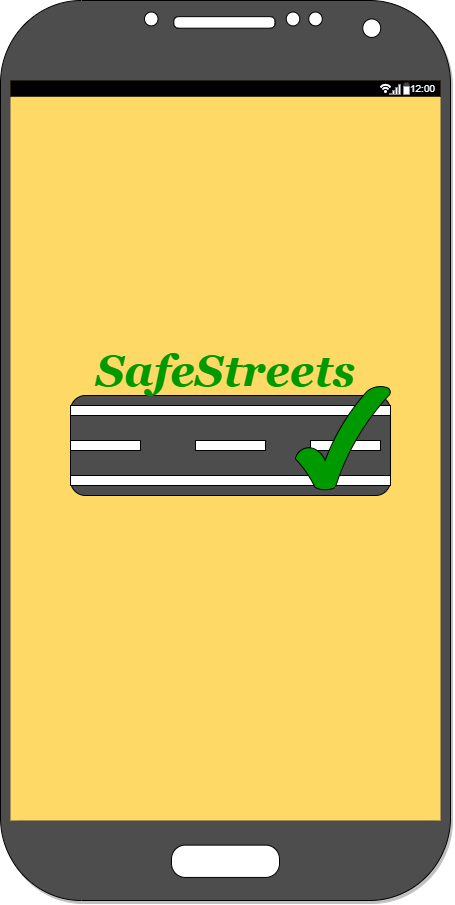
\includegraphics[scale=0.3]{Mockups/Introduction.png}
	\centering
	\caption{SafeStreets Loading}
	\end{figure}
		
		
	\end{itemize}
	
	
	
	
	
	
\end{itemize}

\end{document}


